\documentclass[12pt]{article}

\title{Flatness of control systems}
\date{October 31, 475}
\author{Ciro D. Santilli}

\usepackage{main}

\newcommand{\HRule}{\rule{\linewidth}{0.5mm}}

\begin{document}

\begin{titlepage}
\begin{center}

\includegraphics[width=0.15\textwidth]{ecole_polytechnique_paristech_logo}\\[1cm]
\textsc{\LARGE École Polytechnique}\\[1.5cm]
\textsc{\Large M1 Internship report}\\[0.5cm]
% Title
\HRule \\[0.4cm]
{ \huge \bfseries Flatness in control systems}\\[0.4cm]
\HRule \\[1.5cm]
% Author and supervisor
\begin{minipage}{0.4\textwidth}
\begin{flushleft} \large
\emph{Author:}\\
Ciro D. Santilli
\end{flushleft}
\end{minipage}
\begin{minipage}{0.4\textwidth}
\begin{flushright} \large
\emph{Supervisor:} \\
Jean-Baptiste Pommet
INRIA
\end{flushright}
\end{minipage}
\vfill
% Bottom of the page
{\large Internship period:

from April 9, 2012 to July 6, 2012

\vspace{10 mm}

Report handed in:

July 3, 2012 }

\end{center}

\end{titlepage}

\begin{abstract} Flatness is a desirable property enjoyed by certain control systems.
  If a given control system is flat on a region, then trajectories can be planned in
  a stable way (robust to measurement imprecisions and small random oscillations).
  The main problem today is that it is difficult to determine if a system is flat or
  not, because if a flat output cannot be found by trial and error, and the system
  satisfies all the necessary criteria for flatness, one cannot determine if is flat
  or not. As it turns out, even very simple differential systems made up only out of
  polynomial vector fields have undetermined flatness. This work is an overview
  of the field, presenting the most promising clues that might lead to more general
  answers to the questions in flatness and better algorithms to find flat outputs
  for restricted sets of vector fields (such as the polynomial vector fields).
\end{abstract}

\newpage

\tableofcontents

\newpage

\section{Introduction}

This rapport has been written as the result of a 3 months internship at INRIA Sophia
Antipolis under the supervision of M. Jean Baptiste Pommet, in order for the obtention of a Masters 1 degree at the Ecole Polytechnique
in the domain of applied mathematics.

The goal of the internship was the familiarization with the notion of flatness in particular concerning

\begin{itemize}

  \item its applications to control theory once the flat output is known
  
  \item necessary conditions for flatness, which allow at once to determine
  that some systems are not flat thus saving the non-trivial job of finding
  a flat output.
  
  \item understanding the infinite dimensions point of view, in which generalizes
  the concept of flatness is most elegant to state.
  
\end{itemize}

The ultimate goal of research on this theme, and thus in theory of an internship on the theme of flatness
would either be to find new necessary conditions of flatness, or efficient algorithms that find a
flat output if one exist.

However, it must be noted that the subject is very mathematical, and as such reaching new results requires
an enormous amount of knowledge, which is impossible to obtain in 3 months time. Therefore, the focus of
the internship has been to learn a broad basis on the subject, following many of the clues which might in
the future lead to more satisfactory answers to the question of flatness.

The exposition is organized in the following order:

\begin{enumerate}
  \item the interest behind the concept of flatness is given in \ref{interestOfFlatness}. The major point is the ability to control a system
  once its flatness has been determined.
  
  \item the definition of the concept of flatness given in \ref{def:flatSystem}

  \item examples of systems which are known to be flat, and detailed proofs of that
  are given from \ref{trivial1DControlSystem} onwards.
  
  \item the relationship between flatness and feedback is explained in \ref{flatnessAndFeedback}. The interest here is that a flat system can be put into linear form by a dynamic feedback, and once in linear form, it can be controlled in a stable way. Also, the operation of dynamic feedback is implementable in practice.
 
  \item known necessary conditions for flatness are given in \ref{necessaryConditionsForFlatness}. Those conditions are interesting because if a system satisfies those conditions then no time needs to be wasted to try and transform the system into a flat system.
  
  Also, it is possible that new stronger conditions be built on top of the existing ones.
  
\item in \ref{secInfiniteDimesionSpace} infinite dimension space point of view is
 exposed. It is from this point of view in which definitions for flatness and
 theorems can be stated with the greatest ease.
 
 This point of view suffers an initially high learning curve, and from the fact that
 the results obtained in the end are the same without it as of now.
 
 However, due to its elegance, in the future this may prove to be a possible setting
 to develop new results for the theory of flatness 
 
\end{enumerate}

\subsection{Literature review}

The main sources used for the internship were \cite{MR99} and \cite{Le09}

\begin{itemize}

\item \cite{MR99} contains a more succinct introduction to the subject, which is at the same time quite broad and not extremely deep

\item \cite{Le09} is a much deeper and comprehensive text, which takes
a non compromising approach to the infinite dimension approach explained
in \label{secInfiniteDimesionSpace}. As a consequence, it is a text much
more difficult to completely master, but which gives many examples, and
puts the concepts in an elegant setting.

\end{itemize}

In general, there are not many good introductory books on this subject, in part due to
the fact that it is a quite recent area, dating mostly from around 1990,
and secondly because of the difficulty of algorithmically finding the actual flat output of a system.

\subsection{Motivation and challenge}

\begin{remark}[Interest of flatness]\label{interestOfFlatness}

  Flatness is a desirable property possessed by some control systems 
  
  If a system is flat then it enjoys the fundamental property that
  \begin{itemize}
    \item trajectories can be planned in a stable way
  \end{itemize}
  
  By stable, it is meant that despite measure and random noise perturbations, if
  flatness is present then the system can still be taken from the initial state to
  the desired final state in a robust manner.
  
  The reason behind this is that for a non-linear flat system there is a local
  change of coordinates that locally transforms the system into a linear
  control system, for which the above properties hold. This is shown in
  \ref{flatImpLinDynFeedback}.
\end{remark}

\begin{open-question}[Is there an efficient algorithm to determine the flatness of a system? (open as of 30/05/2012)]
  Once a flat output has been given, it is easy to verify that the system is actually flat.
  
  On the other hand, proving that a system is not flat, even for very restricted
  sets of systems such as those determined by polynomial equations is an open problem in general.
  
  Some necessary conditions are known, but even for very simple systems composed
  only of polynomials those necessary conditions do not suffice.
\end{open-question}

\begin{example}[Simple system with undetermined flatness]
  It is not known if the following system are flat or not (taken from \cite{AP05} as
  of 30/05/2012):
  \begin{align*}
      \dot{z} = y + (\dot{y} - z \dot{x})( \dot{y} - (z-1)\dot{x} )
  \end{align*}
  and
  \begin{align*}
      \dot{z} = y + (\dot{y} - z \dot{x}) \dot{x}
  \end{align*}
  Note how simple those systems are, the associated vector field consisting only of the
  operations of sum and multiplication.
\end{example}

\section{Definition of flatness}

\begin{definition}[Flat system]\label{def:flatSystem}
  A system
  \begin{equation}\begin{aligned}\label{eqControlSystem}
    \dot{x} = f(x,u)
  \end{aligned}\end{equation}
  with state $x \in X \subset \R^n$ and control $u \in U \subset \R^m$ is said to be \emph{flat} iff
  \[ \exists (r,q) \in \N^2 \]
  large enough and
  \[ \exists \funcDom{h}{X \times U \times \R^r}{\R^m}  \]
  and
  \begin{equation}\begin{aligned}
    &\exists \phi \in \COne((\R^m)^{q+1},\R^n) \\
    &\exists \alpha \in \COne((\R^m)^{q+1},\R^m)
  \end{aligned}\end{equation}
  such that
  \begin{enumerate}
  
    \begin{equation}\begin{aligned}
      \forall x \in \COne(\R,X) \\
      \forall u \in \COne(\R,U) \\
    \end{aligned}\end{equation}
    which solve \eqref{eqControlSystem}
  
    \item \label{itm:defFlatOne} the choice
    \begin{equation}\begin{aligned}
    y(t) = h(x(t),u(t),\dot{u}(t),\ldots,u^{(r)}(t))
    \end{aligned}\end{equation}
    implies that
    \[ x(t) = \phi(y(t),\dot{y}(t),\ldots,y^{(q)}(t)) \]
    \[ u(t) = \alpha(y(t),\dot{y}(t),\ldots,y^{(q)}(t)) \]
    
    \item \label{itm:defFlatTwo} there is a single $y$ regular
    \begin{equation}\begin{aligned}
      \exists ! y \in \COne(\R, \R^m)
    \end{aligned}\end{equation}
    such that
    \[ x(t) = \phi(y(t),\dot{y}(t),\ldots,y^{(q)}(t)) \]
    \[ u(t) = \alpha(y(t),\dot{y}(t),\ldots,y^{(q)}(t)) \]
  
  \end{enumerate}
  
\end{definition}

\begin{definition}[Flat output]\label{def:flatOutput}
  The $y$ in \ref{def:flatSystem}, when it exists, is called a \emph{flat output}
  for the system.
\end{definition}

\begin{remark}[Intuition behind the definition of flatness \ref{def:flatSystem} ]
  When stated in plain English, the definition of flatness says two main things:
  \begin{enumerate}
    \item choosing some $y$ though $h$ always generates a solution, so that if we
    ever find an $y$ which will follow a desired trajectory, we can just put it
    inside $h$ and the result will actually be a valid trajectory.
    
    \item that for each solution $(x,u)$ , there exists one, and only one choice of
      $y$ which generates this pair $(x,u)$ through $\phi$ and $\alpha$.
      
      The importance of this point, is that if a desired trajectory is that is
      possible is given, then the function $\alpha$ immediately tells us which 
      $y$ must be chosen in order to follow this trajectory.
  \end{enumerate}
  
  The situation here is analogous to that of a parametrization. For example, in order
  to parametrize a circle $C$ on the plane, one needs to find two functions $x(t)$ and
  $y(t)$ such that for all given $t$
  \begin{itemize}
    \item $(x(t),y(t)) \in C$
    \item $\forall x \in C, \; \exists t, (x(t),y(t)) = x$
  \end{itemize}
  The main difference being that in the case of flatness, it is also required that 
  only a single $t$ should reach every point (cannot go around the circle many times)

  Another strong analogy, is that between flatness and the Brunovsky normal form.
  As in flatness, the Brunovsky normal form is a change of coordinates for linear
  systems, such that in the new coordinates $y$, any choice of $y$ is acceptable,
  and will lead to a trajectory in the original coordinates $x$. For an introduction
  to the subject of the Brunovsky normal form, see \cite{BC11}.

\end{remark}

\section{Examples of flat systems}

\begin{example}[The trivial 1D control system is flat]\label{trivial1DControlSystem}
  The system
  \begin{equation}\begin{aligned}
    \dot{x} = u
  \end{aligned}\end{equation}
  if flat.
\end{example}
\begin{proof}[ Proof  of \ref{trivial1DControlSystem} ]
  Following the notation of the definition \ref{def:flatSystem}, we shall choose
  \begin{equation}\begin{aligned}
    h(x(t),u(t)) &= x(t) \\
    \phi(y(t),\dot{y}(t)) &= y(t) \\
    \alpha(y(t),\dot{y}(t)) &= \dot{y}(t) \\
  \end{aligned}\end{equation}
  So that $r=0$ and $q=1$ will be sufficient, and we will check that this satisfies the two points \ref{itm:defFlatOne}) and \ref{itm:defFlatTwo}) of the definition.
  
  Point \ref{itm:defFlatOne})
  \begin{equation}\begin{aligned}
    y(t) &= h(x(t),u(t)) = x(t) \\
    x(t) &= \phi(y(t),\dot{y}(t)) = y(t) \\
    u(t) &= \alpha(y(t),\dot{y}(t)) = \dot{y}(t)
  \end{aligned}\end{equation}
  implies that
  \begin{equation}\begin{aligned}
    \phi(y(t),\dot{y}(t)) &= y(t) = h(x(t),u(t)) = x(t) \\
    \alpha(y(t),\dot{y}(t)) &= \dot{y}(t) = \dot{x}(t) = u(t)
  \end{aligned}\end{equation}
  
  Point \ref{itm:defFlatTwo}) It is clear that there is a single $y$ for each choice of $(x,u)$, since once $(x,u)$ is fixed we will need to find $y$ such that
  \begin{equation}\begin{aligned}
    x(t) = \phi(y(t),\dot{y}(t)) = y(t)
    u(t) = \alpha(y(t),\dot{y}(t)) = \dot{y}(t)
  \end{aligned}\end{equation}
  which immediately shows that for each $x$ there is one and only one
  choice possible choice of of $y$. But then, $x$ also determines $u$,
  since $u=\dot{x}$, so that for each pair $(x,u)$ there is a single 
  possible $y$
  
\end{proof}

\begin{example}[The trivial 2 states and 1 control system is flat]\label{trivial2DControlSystem}
  The system
  \begin{equation}\begin{aligned}
    \ddot{x} = u
  \end{aligned}\end{equation}
  if flat.
\end{example}
\begin{proof}[ Proof  of \ref{trivial1DControlSystem} ]
  First we put the system on the normal form
  \begin{equation}\begin{aligned}
    \dot{x}_1 &= x_2 \\
    \dot{x}_2 &= x_1 \\
  \end{aligned}\end{equation}
  
  Then using the notations of the definition \ref{def:flatSystem} we will check that
  \begin{equation}\begin{aligned}
    h( (x_1(t),x_2),u(t)) &= x_1(t) \\
    \phi(y, \dot{y}, \ddot{y}) &= \begin{pmatrix} y \\ \dot{y} \end{pmatrix} \\
    \alpha(y, \dot{y}, \ddot{y}) &=  \ddot{y} \\
  \end{aligned}\end{equation}
  works, so that so that $r=0$ and $q=2$ will be sufficient.
  
  Point \ref{itm:defFlatOne}) With
  \begin{equation}\begin{aligned}
    y &= h( x_1, x_2, u) = x_1 \\
    \begin{pmatrix} x_1 \\ x_2 \end{pmatrix}
    &= \phi(y, \dot{y}, \ddot{y})
    = \begin{pmatrix} y \\ \dot{y} \end{pmatrix} \\
    \alpha(y,\dot{y},\ddot{y}) &= \ddot{y}
  \end{aligned}\end{equation}
  we have it that
  \begin{equation}\begin{aligned}
    \phi_1(y,\dot{y},\ddot{y}) &= y = h(x_1,x_2,u) = x_1 \\
    \phi_2(y,\dot{y},\ddot{y}) &= \dot{y} = \dot{x}_1 = x_2 \\
    \alpha(y,\dot{y},\ddot{y}) &= \ddot{y} = \ddot{x}_1 = \dot{x}_2 = u
  \end{aligned}\end{equation}
  
  Point \ref{itm:defFlatTwo}) If we fix a solution $(x,u)$, then $y$ is
  given by
  \begin{equation}\begin{aligned}
    y = x_1
  \end{aligned}\end{equation}
  so that for each $x$, there is only one possible choice for $y$, that
  is, $y=x_1$.
  Also, $u$ is determined by the choice of $x$, which means that for
  each pair $(x,u)$ there is only one possible choice of $y$. 
\end{proof}

\begin{remark}[Trivial systems]
  What has been done on \ref{trivial1DControlSystem} and \ref{trivial2DControlSystem} can be easily generalized to any system of
  degree $n$ of the form
  \begin{equation}\begin{aligned}
    \dot{x}_1 &= x_2 \\
    \dot{x}_2 &= x_1 \\
    &\ldots \\
    \dot{x}_n &= u \\
  \end{aligned}\end{equation}
  which will be flat with flat output $x_1$.
  
  This type of system is so simple that it gets a special name: the trivial system.
\end{remark}

\begin{example}[Double serial mass spring non-linear damper] \label{expTwoMassParallel} \label{exp:controllingNonLinearSystem}
  The non-linear system taken from \cite[p.133]{Le09}
  \begin{equation}\begin{aligned} \label{eq2}
    &\ddot{x}_1 = c_1 x_1 + c_2 x_2 + f_1(\dot{x}_1) \\
    &\ddot{x}_2 = c_3 x_1 + c_4 x_2 + f_2(\dot{x}_2) + c_5u
  \end{aligned}\end{equation}
  with non-linear friction terms $f_i$, states $x_i$, control $u$ and $c_i$ constants is flat.
  This equations can model a two serial mass spring non-linear dumper system represented in \figRef{figDoubleMassSpringSystem}
  \begin{figure}[h]
    \centering  
    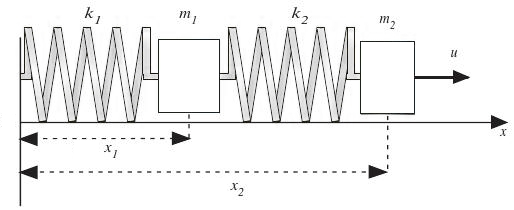
\includegraphics{double_spring_mass_dumper_levine_p133_bw_simplified}
    \caption{Double spring mass non-linear dumper system}
    \label{figDoubleMassSpringSystem}
  \end{figure}  
  where $m_i$ are the masses, $k_i$ are the linear elastic constants, and $f_i$ are the non-linear friction terms, and the constants are given as
  \begin{equation}\begin{aligned}
    c_1 &= \frac{k_1 + k_2}{m_1} \\
    c_2 &= - \frac{k_2}{m_2} \\
    c_3 &= \frac{1}{m_2} \\
    c_4 &= -\frac{k_2}{m_2} \\
    c_5 &= \frac{1}{m_2}
  \end{aligned}\end{equation}
\end{example}
\begin{proof}[ Proof of \ref{expTwoMassParallel}]
  First we put the system on the normal form
  \begin{equation}\begin{aligned}
    \ddot{x}_1 &= x_3 \\
    \ddot{x}_2 &= x_4 \\
    \ddot{x}_3 &= c_1 x_1 + c_2 x_2 + f_1(\dot{x}_1) \\
    \ddot{x}_4 &= c_3 x_1 + c_4 x_2 + f_2(\dot{x}_2) + c_5u    
  \end{aligned}\end{equation}
  and we will show that
  \begin{equation}\begin{aligned}
    h(x(t),u(t)) &= x_1(t) \\
    \phi(y, \dot{y}, \ddot{y}, y^{(3)} ) &=
    \begin{pmatrix}
      y \\
      \frac{1}{c_2} ( c_1 y + f_1(\dot{y}) + \ddot{y} \\
      \dot{y} \\
      \frac{1}{c_2} ( c_1 \dot{y} + \der{}{\dot{y}} [f_1(\dot{y})]\ddot{y} + y^{(3)}
    \end{pmatrix}
  \end{aligned}\end{equation}
  is a flat output.
  This time, we are not going to give $\phi$ and $\alpha$ explicitly, because their
  full expression would be too long and uninformative, but we will show how to
  calculate them.
  
  Point \ref{itm:defFlatOne}) In order to determine $\phi$ and $\alpha$ we are
  going to need to put all the state variables as a function of $y = h(x,u) = x_1$ and its derivatives.
  Immediately, the two state variables $x_1$ and $x_3 = \dot{x}_1$ are a function of $x_1$
  and its derivative $\dot{x}_1$, so we are done for them, having determined two components of the function $\phi$
  \begin{equation}\begin{aligned}
    \phi_1(y, \dot{y}, \ddot{y}, y^{(3)}) &= y = x_1 \\
    \phi_3(y, \dot{y}, \ddot{y}, y^{(3)}) &= \dot{y}
  \end{aligned}\end{equation}

  Next,
  \begin{equation}\begin{aligned} \label{eq1}
    x_2 &= \frac{1}{c_2} ( c_1 x_1 + f_1(\dot{x}_1) + \ddot{x}_1 ) \\
    &=  \frac{1}{c_2} ( c_1 y + f_1(\dot{y}) + \ddot{y} )
  \end{aligned}\end{equation}
  so $x_2$ could be expressed in terms of $x_1$ and its derivatives, and thus in 
  terms of $y$ and its derivatives, which implies
  \begin{equation}\begin{aligned}
    \phi_2(y, \dot{y}, \ddot{y}, y^{(3)}) =  \frac{1}{c_2} ( c_1 y + f_1(\dot{y}) + \ddot{y})
  \end{aligned}\end{equation}
  Therefore, in order go express $x_4$ in terms of the flat output $x_1$, all we have to do is to derive the expression obtained for $x_2$ giving
  \begin{equation}\begin{aligned}
    x_4
    &= \dot{x}_2
    = \frac{1}{c_2} ( c_1 \dot{x}_1 + \der{}{\dot{x}} [f_1(\dot{x}_1)]\ddot{x}_1 + x_1^{(3)} ) \\
    &= \frac{1}{c_2} ( c_1 \dot{y} + \der{}{\dot{y}} [f_1(\dot{y})]\ddot{y} + y^{(3)} )
  \end{aligned}\end{equation}
  meaning that
  \begin{equation}\begin{aligned}
    \phi_4(y, \dot{y}, \ddot{y}, y^{(3)}) = \frac{1}{c_2} ( c_1 \dot{y} + \der{}{\dot{y}} [f_1(\dot{y})]\ddot{y} + y^{(3)}
  \end{aligned}\end{equation}
  which has finished determining $\phi$.
  
  Finally, it is also easy to express $u$ in terms of the flat output $x_1$, because
  from \eqref{eq2} we have it that
  \begin{equation}\begin{aligned}
    u = \frac{1}{c_5}[ \ddot{x}_2 - c_3 x_1 - c_4 x_2 - f_2(\dot{x}_2) ]
  \end{aligned}\end{equation}
  so it is all a matter of deriving $\dot{x}_2$ again, which in turn shows us that
  we would need up to the fourth derivative of $x_1$ for $\alpha$.
  
  Point \ref{itm:defFlatTwo}) If $(x,u)$ is a solution then we have $y = x_1$, so
  that there is at most one possible $y$ for each solution, since $x_1$ then
  determines $x_2$ and $u$.
  Also, it is clear that the choice $y=x_1$ really gives the only solution, because
  in Point 1) it has been shown that $x=\phi(y,\dot{y},\ddot{y},y^{(3)})$ and
  $u=\alpha(y,\dot{y},\ddot{y},y^{(3)},y^{(4)})$ under the choice $x_1$.
\end{proof}

\begin{remark}[on \ref{expTwoMassParallel}]
  The flat output often is a remarkable physical property of the system. In \ref{expTwoMassParallel} this is very
  clear since the flat output is directly the position of the first mass.
\end{remark}

\begin{example}[Vertical plane take-off] \label{expVertPlaneTakeoff}
  The equations
  \begin{equation}\begin{aligned} \label{eq5}
    \ddot{x}_1 &= -u_1 \sin{x_3} + a u_2 \cos{x_3} \\
    \ddot{x}_2 &= u_1 \cos{x_3} + a u_2 \sin{x_3} - 1 \\
    \ddot{x}_3 &= u_2
  \end{aligned}\end{equation}
    can model the take-off of a plane.
    
    We claim that this system is flat, with flat outputs (defined \ref{def:flatOutput}) given by
    \begin{align}
      y =
      \begin{pmatrix}
        x_1 - a \sin{x_3} \\
        x_2 + a \cos{x_3}
      \end{pmatrix}
    \end{align}
\end{example}
\begin{proof}[ Proof of \ref{expVertPlaneTakeoff}]
  Note that
  \begin{align}
    (y_1 - x_1) &= - a \sin{x_3} \\
    (y_2 - x_2) &= a \cos{x_3} \\
    \ddot{y}_1 &= \ddot{x}_1 + a[ \sin{x_3} \dot{x}_3^2 - \cos{x_3} \ddot{x}_3 ] \\
    \ddot{y}_2 &= \ddot{x}_2 + a[ \cos{x_3} \dot{x}_3^2 + \sin{x_3} \ddot{x}_3 ]
  \end{align}
  which implies
  \begin{align}
    (y_1 - x_1)^2 + ( y_2 - x_2 )^2 &= a^2 \label{eq2} \\
    (y_1 - x_1)(\ddot{y}_2 + 1 ) -  ( y_2 - x_2 )\ddot{y}_1 &= 0 \label{eq3} \\
    (\ddot{y}_2 + 1 ) \sin{\theta} + \ddot{y}_1 \cos{\theta} &= 0 \label{eq4}
  \end{align}
  After some more algebraic exercise, we find it that \eqref{eq2} and \eqref{eq3} imply
  \begin{align}
    x_1 &= y_1 \pm a \frac{\ddot{y}_1}{\sqrt{\ddot{y}_1 + (\ddot{y}_2 + 1)^2 }} \\
    x_2 &= y_2 \pm a \frac{\ddot{y}_2 + 1}{\sqrt{\ddot{y}_1 + (\ddot{y}_2 + 1)^2 }} 
  \end{align}
  and that \eqref{eq4} implies that
  \begin{align}
    x_3 = \arctan{ \left( \ddot{y}_2 + \frac{1}{\ddot{y}_1} \right)}
  \end{align}
  So that we have put all the state variables in terms of $y_i$,
  since we only need to differentiate to find
  the missing $\dot{x}_i$.
  
  Note that there is a single singularity when $\sqrt{\ddot{y}_1 + (\ddot{y}_2 + 1)^2}$
  
  Also the controls can be put in terms of the state variables since from \eqref{eq5}, it follows that
  \begin{align}
    u_2 &= \ddot{x}_3 \\
    u_1 &= \frac{\ddot{x}_2 - a u_2 \sin{x_3} + 1}{\cos{x_3}}
  \end{align}
\end{proof}

\begin{example}[Non-holonomic vehicle] \label{expNonHoloVehicle}
  The system
  \begin{equation}\begin{aligned}
    \dot{x}_0 &= u_1 \cos{\theta_0} \\
    \dot{y}_0 &= u_1 \sin{\theta_0} \\
    \dot{\theta}_0 &= \frac{u_1}{d_0} \tan{\phi} \\
    \dot{\theta}_i &= \frac{u_1}{d_i} \left( \prod_{j=1}^{i-1} \cos{\theta_{j-1} - \theta_i} \right) sin ( \theta_{j-1} - \theta_j ) & i \in [1 ..  n]
  \end{aligned}\end{equation}
  where $x_n$, $y_n$ and $\theta_i$ are state variables and $u$ and $\phi$ are the controls.
  is flat with flat output $(x_n, y_n)$.
  The equations can model a non-holonomic n-trailer vehicle as shown in \figRef{figNonHoloVehicle}
  
  \begin{figure}[h]
    \centering
    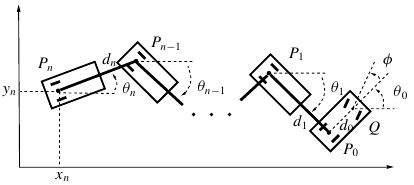
\includegraphics{non_holonomic_ntrailler}
    \caption{Non-holonomic n-trailer}
    \label{figNonHoloVehicle}
  \end{figure}
  
  where the state variables $x_n$, $y_n$ and $\theta_i$ correspond respectively to the
  positions and angles of each car, and the controls $u$ and $\phi$ correspond to the
  velocity of the first car, and the angle of the wheels of the first car,
  and the $d_i$ are the constant lengths of each axe.
  
  Note that all the other $x_i$ and $y_i$ do not need to be added to the state
  because they can be determined in terms of $(x_n,y_n)$ by
  \begin{equation}\begin{aligned}
    x_{n-1} &= x_n + d_n cos \theta_n \\
    y_{n-1} &= y_n + d_n sin \theta_n
  \end{aligned}\end{equation}  

  The system is said to be nonholonomic because a holonomic system is one described
  without the use of derivatives, while this one has the derivatives explicit on the
  equation.
\end{example}
\begin{proof}[ Proof of \ref{expNonHoloVehicle}]
  We will put each state and control in function of the flat output $(x_n,y_n)$.
  
  To do so, we will recurse, from $(x_n,y_n)$ down to the lowest $(x_0,y_0)$, which
  will allow to determine all the states.

  First note that
  \begin{equation}\begin{aligned} \label{eqThetaNFuncXnYn}
    \theta_{n} = \frac{\dot{y}_n}{\dot{x}_n}
  \end{aligned}\end{equation}
  which means that $\theta_n$ could be put in function of our flat outputs $(x_n,y_n)$. 
  \eqref{eqThetaNFuncXnYn} can be easily seen if we denote by $u_i$ the speed of the
  ith car, since we have then:
  \begin{equation}\begin{aligned}
    \dot{x}_i &= u_i cos \theta_i \\
    \dot{y}_i &= u_i cos \theta_i
  \end{aligned}\end{equation}
  and then we just have to divide those two equations, so the value of $u_i$ doesn't matter here.
  
  Next, we can also express the lower $x_{n-1}$ and $y_{n-1}$ in terms of the higher
  order terms which have already been determined by
  \begin{equation}\begin{aligned}
    x_{n-1} &= x_n + d_n cos \theta_n \\
    y_{n-1} &= y_n + d_n sin \theta_n
  \end{aligned}\end{equation}
  which in turn allows us to determine the lower degree state variable
  \begin{equation}\begin{aligned}
    \theta_{n-1} = \frac{\dot{y}_{n-1}}{\dot{x}_{n-1}}
  \end{aligned}\end{equation}
  so that all the $\theta_i$ can be put in this manner as a function of $(x_n,y_n)$
  
  All that is left is to determine the control $u$ in function of known terms, but
  this is simple since from the original system we have that
  \begin{equation}\begin{aligned}
    u = \frac{\dot{x}_0}{cos \theta_0}
  \end{aligned}\end{equation}
  
\end{proof}

\section{Flatness and feedback} \label{flatnessAndFeedback}

\begin{remark}[Flatness and feedback]
  One major advantage of flatness is that if a system is flat, then it can be transformed into a linear system,
  through a process called linearisation by dynamic feedback (defined in \ref{defLinDynFeedback}). \ref{flatImpLinDynFeedback}
  proves that this is actually possible.  
  
  The interest of this is that linearisation by
  dynamic feedback is an operation that is is implementable in practice, so that flat systems can be made
  linear and treated with the very strong linear techniques in practice.
\end{remark}

\begin{definition}[Static feedback] \label{defStaFeedback}
  A static feedback is a pair of functions $a$ and $b$ which transforms a system
  \begin{equation}\begin{aligned}
    \dot{x} = f(x,u)
  \end{aligned}\end{equation}
  with state $x$ and control $u$ as
  \begin{equation}\begin{aligned}
    y = a(x)
    v = b(x,u)
  \end{aligned}\end{equation}
  so that $y$ will be the new state, and $v$ will be the new control of the transformed system.
\end{definition}

\begin{definition}[Dynamic feedback] \label{defDynFeedback}
  A \emph{feedback} is a pair of functions $g$ and $h$, which transform the system
  \begin{equation}\begin{aligned}
    \dot{x} = f(x,u)
  \end{aligned}\end{equation}
  with state $x$ and control $u$ into
  \begin{equation}\begin{aligned}
    \dot{x} &= f(x,g(x,z,v))) \\
    \dot{z} &= h(x,z,v)
  \end{aligned}\end{equation}
  where $z$ has a free as large as wanted dimension
  \begin{equation}\begin{aligned}
    z &= (z_1, z_2, \ldots, z_n) \\
  \end{aligned}\end{equation}
  Then $z$ has then been added to the state, so that the new state is $(x,z)$, and the old control $u$ has been eliminated by
  \begin{equation}\begin{aligned}
    u = g(x,z,v)
  \end{aligned}\end{equation}
  so that the new control is $v$.
\end{definition}

\begin{definition}[Linearisable by dynamic feedback] \label{defLinDynFeedback}
  A control system is \emph{linearisable by dynamic feedback} iff if can be transformed by a dynamic
  feedback \ref{defDynFeedback} into a system that is linearisable by static feedback \ref{defLinStaFeedback}.
\end{definition}

\begin{definition}[Linearisable by static feedback] \label{defLinStaFeedback}
  A control system is \emph{linearisable by static feedback} iff there exists a static feedback
  \ref{defStaFeedback} such that the transformed system is linear, that is, $\exists A, B$ such that
  \begin{equation}\begin{aligned}
    \dot{y} = Ay + Bv
  \end{aligned}\end{equation}
  where $y$ is the new state, and $v$ the new control.
\end{definition}

\begin{theorem}[Flat implies linearisable by dynamic feedback] \label{flatImpLinDynFeedback}
  A flat system can be linearised by dynamic feedback \ref{defLinDynFeedback}.
\end{theorem}
\begin{proof}
  See \cite[page 50, corollary 3.15]{MR99}
\end{proof}

\begin{example}[ of \ref{flatImpLinDynFeedback}. Vertical plane take-off ] \label{expVertPlaneTakeoffLin}
  Take the system
  \begin{equation}\begin{aligned} \label{eq5}
    \ddot{x}_1 &= -u_1 \sin{x_3} + a u_2 \cos{x_3} \\
    \ddot{x}_2 &= u_1 \cos{x_3} + a u_2 \sin{x_3} - 1 \\
    \ddot{x}_3 &= u_2
  \end{aligned}\end{equation}
  which as we have seen in \ref{expVertPlaneTakeoff} is flat with flat output
  \begin{align}
    y =
    \begin{pmatrix}
      x_1 - a \sin{x_3} \\
      x_2 + a \cos{x_3}
    \end{pmatrix}
  \end{align}
  Then the following dynamic feedback ( defined in \ref{defDynFeedback} ) with $z \in \R^2$
  \begin{equation}\begin{aligned}
  	g(x,z,v)
    &= \begin{pmatrix} u_1 \\ u_2 \end{pmatrix}
    = \begin{pmatrix} z_1 + a \dot{x}_3^2 \\ -\frac{1}{z_1}(v_1 \cos{x_3} + v_2 \sin{x_3} + 2 z_2 \dot{x}_3) \end{pmatrix}
    \\
    h(x,z,v)
    &= \begin{pmatrix}\dot{z}_1 \\ \dot{z}_2 \end{pmatrix}
    = \begin{pmatrix}z_2 \\ -v_1 \sin{x_3} + v_2 \cos{x_3} + z_1\dot{x_3}^2 \end{pmatrix}
  \end{aligned}\end{equation}
  where we remember that $\dot{\theta}$ is part of the state of the original equation, followed by the change of coordinates
  \begin{equation}\begin{aligned}
    \begin{pmatrix}
      x_1 \\ x_2 \\ x_3 \\ \dot{x}_1 \\ \dot{x}_2 \\ \dot{x}_3 \\ z \\ \dot{z}
    \end{pmatrix}
    \mapsto
    \begin{pmatrix}
      y_1 \\ y_2 \\ \dot{y}_1 \\ \dot{y}_2 \\ \ddot{y}_1 \\ \ddot{y}_2 \\ y_1^{(3)} \\ y_2^{(3)}
    \end{pmatrix}
  \end{aligned}\end{equation}
  puts the system in linear form
  \begin{equation}\begin{aligned}
    y_1^{(4)} &= v_1 \\
    y_2^{(4)} &= v_2
  \end{aligned}\end{equation}
\end{example}

\begin{proof}[ Proof of \ref{expVertPlaneTakeoffLin}]
  TODO17
\end{proof}

\section{Known necessary conditions for flatness} \label{necessaryConditionsForFlatness}

In this section we will show that the specific system \eqref{eq:reimanSystem} is
not flat.

\subsection{Flat implies ruled}

\begin{remark}[Flat implies ruled]
  A flat system must be ruled (defined in \ref{def:ruledSystem}) as shown in  \ref{theoFlatImpliesRuled}.
  This may be useful to prove that certain systems are not flat in a simple manner if they are not ruled,
  as illustrated in \ref{expSysNotRuled}.
\end{remark}

\begin{definition}[Ruled system] \label{def:ruledSystem}
  Given a control system, we can eliminate the $u_i$ locally by the inverse function theorem,
  giving $n-m$ equations of the type
  \begin{equation}\begin{aligned}
    F_i(x,\dot{x}) = 0 \\
    i \in \{1 .. n-m\}
  \end{aligned}\end{equation}
  A control system is said to be \emph{ruled} iff after the elimination of the $u_i$, for each
  $F_i$ and pair $(x,p)$ such that $F_i(x,p)=0$ there exists $a \in \R_\star^n$ such that for all $\lambda$
  \begin{equation}\begin{aligned}
    F(x, p + a\lambda) = 0
  \end{aligned}\end{equation}
  Informally, this means that for each point, there passes a straight line which is
  entirely contained in the variety.
\end{definition}

\begin{theorem}[Flat implies ruled (defined in \ref{def:ruledSystem})] \label{theoFlatImpliesRuled}
\end{theorem}
\begin{proof}[ Proof of \ref{theoFlatImpliesRuled}]
  The proof can be found in \cite[p.58, theorem 3.26]{MR99}
\end{proof}

\begin{example}[A system that is not flat because it is not ruled] \label{expSysNotRuled}
  The following system
  \begin{equation}\begin{aligned}
    \dot{x}_1 &= u_1 \\
    \dot{x}_2 &= u_2 \\
    \dot{x}_3 &= u_1^2 + u_2^3 \\
  \end{aligned}\end{equation}
  is not flat because it is not ruled (as defined in \ref{def:ruledSystem}).
\end{example}
\begin{proof}[ Proof of \ref{expSysNotRuled}]
  By eliminating $u_1$ and $u_2$, we reach
  \begin{equation}\begin{aligned}
    &\dot{x}_3 = \dot{x}_1^2 + \dot{x}_2^3 \\
    &\implies \dot{x}_3 - \dot{x}_1^2 - \dot{x}_2^3 = 0
  \end{aligned}\end{equation}
  so $n=3$, $m=2$ and using the notation introduced in the definition
  \ref{def:ruledSystem}, is only one $F_i$
  \begin{equation}\begin{aligned}
    F_1(x,\dot{x}) = \dot{x}_3 - \dot{x}_1^2 - \dot{x}_2^3
  \end{aligned}\end{equation}
  Now take a value of the derivative $\dot{x}=p$ such that
  \begin{equation}\begin{aligned}
    F_1(x,p) = 0  
  \end{aligned}\end{equation}
  which is the same as saying that
  \begin{equation}\begin{aligned}
    p_3 - p_1^2 - p_2^3 = 0
  \end{aligned}\end{equation}
  suppose we can find $a \in \R^3$ such that for any $\lambda \in \R$
  \begin{equation}\begin{aligned}
    F_1(x,p + \lambda a) = 0 
  \end{aligned}\end{equation}
  We will proceed to show that this implies that $a=0$, not satisfying then the definition of ruled system, which requires $a \in \R_\star^n$.
  
  We have that for any $\lambda \in \R$
  \begin{equation}\begin{aligned}
    p_3 + \lambda a_3 - (p_1 + \lambda a_1)^2 - (p_2 + \lambda a_2)^3 = 0
  \end{aligned}\end{equation}
  Expanding the powers, we get it that
  \begin{equation}\begin{aligned}
    &p_3 + \lambda a_3 \\
    &- [(p_1)^2 + 2(p_1 \lambda a_1) + (\lambda a_1)^2] \\
    &- [(p_2)^3 + 4(p_2)^2 \lambda a_2 + 6(p_2 + \lambda a_2) + 4 p_2(\lambda a_2)^2 + (\lambda a_2)^3 ] \\
    &= ( p_3 - p_1^2 - p_2^3 ) + \lambda^3 a_2^3 + R(a,p,\lambda) \\
    &= 0 + \lambda a_3 + \lambda^3 a_2^3 + R(a,p,\lambda) \\
    &= 0 \\
  \end{aligned}\end{equation}
  where the rest $R$ is a multinomial and contains no terms with $\lambda^3$. Therefore, since the only term in
  $\lambda^3$ is $a_2^3 \lambda ^3$, we must have it that $a_2^3 = 0 $ which implies $a_2 = 0 $.
  
  Isolating then the term in $\lambda^2$, we have only $a_1^2 \lambda^2$, which means that $a_1 = 0$ and finally,
  doing the same for the terms in $\lambda$ that are left, we reach it that $a_3 = 0$.
  
  Therefore we must have $a=0$, and the system is not ruled.
  
\end{proof}

\subsection{A specific case studied by Hilbert} \label{secHilbertCase}

In this section, it shall be shown that the system \eqref{reimanSystem} is not flat.

\begin{historicalRemark} The system \eqref{reimanSystem} was briefly studied by Hilbert.
While the concept of flatness as we know it today was not formulated at his time,
he was already interested in the parametrization of solutions of differential
equations, and his ideas can be used to show that the system is not flat.
\end{historicalRemark}

\begin{remark}[Interest of proving that \eqref{eq:reimanSystem} is not flat]
Even if the system \eqref{eq:reimanSystem} is rather doesn't fall on any on the
more general necessary conditions of flatness. Therefore, even if the proof is specific
for this case only, the idea behind it can be generalized, and it has been an inspiration
for the results presented in \citep{AP05}.
\end{remark}

\begin{proposition} \label{reimanSystem}
The system
\begin{align} \label{eq:reimanSystem}
  \begin{cases}
    \dot{x} &= u_1 \\ 
    \dot{\alpha} &= u_2 \\ 
    \dot{\beta} &= \alpha u_1 \\
    \dot{z} &= \alpha^2 u_1 \\
    \dot{y} &= \beta u_1
  \end{cases}
\end{align}
is not flat.
\end{proposition}

\begin{proof}[ Proof of \ref{reimanSystem}]
For the whole proof, notations \ref{indexIIsForOneAndTwo} and \ref{derivativesOfComplicatedThings} will be assumed.

The proof is broken into several steps:
\begin{enumerate}
  \item simplification. In \ref{simplificationOfReimanSystem} we will prove that
    \eqref{eq:reimanSystem} is flat implies that the simpler system
    \begin{equation}\begin{aligned} \label{reimanSysXYZ}
      \dot{z} (\dot{x})^5 = (\ddot{y}\dot{x} - \dot{y}\ddot{x})^2
    \end{aligned}\end{equation}
    is also flat. Our goal then will be of course to show this simplified system is not flat, that is, it cannot be written in the form
    \begin{equation}\begin{aligned}\label{eq:reimanSystemXYZDefFlat}
  x &= \varphi( w_1, \dot{w}_1, \ldots, w_1^{(\alpha_1)}, w_2, \dot{w}_2, \ldots, w_2^{(\alpha_2)} ) \\
  y &= \phi( w_1, \dot{w}_1, \ldots, w_1^{(\alpha_1)}, w_2, \dot{w}_2, \ldots, w_2^{(\alpha_2)} ) \\
  z &= \chi( w_1, \dot{w}_1, \ldots, w_1^{(\alpha_1)}, w_2, \dot{w}_2, \ldots, w_2^{(\alpha_2)} ) \\
\end{aligned}\end{equation}
    
  \item We make a change of coordinates $x \mapsto w_1^{(\alpha_1)}$ which will put the system \eqref{eq:reimanSystemXYZDefFlat} in the form
\begin{equation}\begin{aligned} \label{eq:reimanSystemFGH}
  y &= f( w_1, \dot{w}_1, \ldots, w_1^{(\alpha_1 - 1)}, x, w_2, \dot{w}_2, \ldots, w_2^{(\alpha_2)} ) \\
  z &= g( w_1, \dot{w}_1, \ldots, w_1^{(\alpha_1 - 1)}, x, w_2, \dot{w}_2, \ldots, w_2^{(\alpha_2)} ) \\
  w_1^{(\alpha_1)} &= h( w_1, \dot{w}_1, \ldots, w_1^{(\alpha_1 - 1)}, x, w_2, \dot{w}_2, \ldots,   w_2^{(\alpha_2)} ) \\
\end{aligned}\end{equation}
    where in accordance with \ref{derivativesOfComplicatedThings} $w_1^{(\alpha_1)}$ denotes a component and not the derivative of a function.
    \ref{changeOfCoordinates} proves that this actually is a change of coordinates.
    
  \item working in the new coordinates, we reach the conclusions that $f$ and $g$ are both a
  function only of $x$, which is is proven in \ref{fDepOnlyX} and \ref{gDepOnlyX}.
  
  \item since $f$ and $g$ are only a function of $x$, once an $x$ is given, then that determines $y$ and $z$ because
  \begin{equation}\begin{aligned}
    y(t) &= f(x(t)) \\
    z(t) &= g(x(t))
  \end{aligned}\end{equation}
  But then it is not possible to cover all possible solutions of \eqref{reimanSysXYZ}.
  This is so because by fixing an $w_i$, this fixes an $x$, which in
  in turn fixes $y$ and $z$. But it is easy to see that for a single
  $x$ there can be many possible solutions $y$ and $z$. For example,
  if we take
  \begin{equation}\begin{aligned}
    x(t) = t
  \end{aligned}\end{equation}
  then both then $\dot{x(t)} = 1$ and thus \eqref{reimanSysXYZ} reduces to
  \begin{equation}\begin{aligned}
    \dot{z} = \ddot{y}^2
  \end{aligned}\end{equation}
  which clearly has an infinity of polynomial solutions, for example
  \begin{equation}\begin{aligned}
    y(t) &= \frac{t^2}{2} \\
    z(t) &= t
  \end{aligned}\end{equation}
  or
  \begin{equation}\begin{aligned}
    y(t) &= \frac{t^3}{6} \\
    z(t) &= \frac{t^3}{3}
  \end{aligned}\end{equation}
  Therefore, not all of the solutions can be covered by choosing $w_i$,
  and the system cannot be flat, since condition \ref{itm:defFlatTwo}) of 
  the definition \ref{def:flatSystem} fails.
\end{enumerate}

Note that some of the steps in the proof are quite technical, but two main simple
techniques are used in the proof:

\begin{enumerate}
  \item taking the derivatives of $\varphi$ and $\phi$ and looking reaching new
  equalities by observing the highest order terms $w^{(\alpha_i + 1)}$ that come out
  \item reaching impossibilities based on the fact that one side of the equalities
  obtained has polynomial dependence of different order than the other side on a
  certain variable (for example one side of the equality depends on $(w^{(\alpha_i + 1)})^2$ while the other on $(w^{(\alpha_i + 1)})$ )
\end{enumerate}

\end{proof}

\begin{notation}[Index $i$] \label{indexIIsForOneAndTwo}
  When the index $i$ is used in the context of the proof of \ref{reimanSystem},
  we will assume that the affirmations are valid for \emph{both} $i=1$ and $i=2$.
\end{notation}

\begin{notation}[Derivatives] \label{derivativesOfComplicatedThings}
  Partial derivatives will be denoted by a subscript, and as a convenient mnemonic device
  each component of the functions $\varphi$, $\psi$ and $\xi$ will be denoted by the same arguments
  as the reference formula \eqref{eq:reimanSystemDefFlat}.
  
  Therefore, for example
  \[ \varphi_{w_1^{(2)}} \]
  denotes the derivative of $\varphi$ with respect to its \emph{third} variable, which is
  usually in our context the argument of \eqref{eq:reimanSystemDefFlat} that is located at that position.
  This has no real relation (except the mnemonic one) to the second derivative of $w_1$.
\end{notation}

\begin{lemma}[Simplification to $x$, $y$ and $z$ only] \label{simplificationOfReimanSystem}

If \eqref{eq:reimanSystem} is flat, then
\begin{align} \label{eq:reimanSystemXYZ}
  \dot{z} (\dot{x})^5 = (\ddot{y}\dot{x} - \dot{y}\ddot{x})^2
\end{align}
is also flat, in the sense that there is $\alpha_1$ and $\alpha_2 \in \N$ and
three functions $\varphi$, $\psi$ and $\chi$ such that for any two functions $w_1(t)$ and $w_2(t)$ the choice
\begin{equation} \label{eq:reimanSystemXYZDefFlat}
\begin{aligned} 
  x &= \varphi( w_1, \dot{w}_1, \ldots, w_1^{(\alpha_1)}, w_2, \dot{w}_2, \ldots, w_2^{(\alpha_2)} ) \\
  y &= \phi( w_1, \dot{w}_1, \ldots, w_1^{(\alpha_1)}, w_2, \dot{w}_2, \ldots, w_2^{(\alpha_2)} ) \\
  z &= \chi( w_1, \dot{w}_1, \ldots, w_1^{(\alpha_1)}, w_2, \dot{w}_2, \ldots, w_2^{(\alpha_2)} ) \\
\end{aligned}
\end{equation}
always satisfies \eqref{eq:reimanSystemXYZ}.
\end{lemma}
\begin{proof}
\eqref{eq:reimanSystem} being flat means that there is $\alpha_1$ and $\alpha_2
\in \N$ and seven functions $\varphi$, $\psi$, $\chi$ and four others such that
for any two functions $w_1(t)$ and $w_2(t)$ the choice
\begin{equation} \label{eq:reimanSystemDefFlat}
  \begin{aligned}
    x &= \varphi( w_1, \dot{w}_1, \ldots, w_1^{(\alpha_1)}, w_2, \dot{w}_2, \ldots, w_2^{(\alpha_2)} ) \\
    y &= \phi( w_1, \dot{w}_1, \ldots, w_1^{(\alpha_1)}, w_2, \dot{w}_2, \ldots, w_2^{(\alpha_2)} ) \\
    z &= \chi( w_1, \dot{w}_1, \ldots, w_1^{(\alpha_1)}, w_2, \dot{w}_2, \ldots, w_2^{(\alpha_2)} ) \\
    \alpha &= \ldots \\
    \beta &= \ldots \\
    u_1 &= \ldots \\
    u_2 &= \ldots \\
  \end{aligned}
\end{equation}
always satisfies \eqref{eq:reimanSystem}.

But \eqref{eq:reimanSystem} implies \eqref{eq:reimanSystemXYZ} because
\[ \dot{z}(\dot{x})^5 = \alpha^2 u_1 (u_1)^5 = \alpha^2 (u_1)^6 \]
and
\begin{align*}
  ( \ddot{y}\dot{x} - \dot{y}\ddot{x} )^2
  &= ( (\dot{\beta}u_1 + \beta \dot{u}_1) u_1 - \beta u_1 (\dot{u}_1) )^2 \\
  &= ( (\alpha u_1) u_1^2 + \beta \dot{u} u_1 - \beta u_1 (\dot{u}_1) )^2 \\
  &= ( \alpha u_1^3 ) ^2 \\
  &= \alpha^2 u_1^6
\end{align*}

Therefore, since if we can find functions that will satisfy \eqref{eq:reimanSystemDefFlat},
in particular we can also find functions $\varphi$, $\psi$ and $\chi$ that satisfy
\eqref{eq:reimanSystemXYZDefFlat}, as stated in \ref{simplificationOfReimanSystem}
\end{proof}

\begin{lemma}[Change of coordinates] \label{changeOfCoordinates}
 The function
 \begin{equation}\begin{aligned}
    \Phi
    \begin{pmatrix}
      p_1 \\ p_2 \\ \ldots \\ p_{\alpha_1 - 1} \\ p_{\alpha_1} \\ q_1 \\ q_2 \\ \ldots \\ q_{\alpha_2}
    \end{pmatrix}
    =
    \begin{pmatrix}
        p_1 \\ p_2 \\ \ldots \\ p_{\alpha_1 - 1} \\ \varphi(pq) \\ q_1 \\ q_2 \\ \ldots \\ q_{\alpha_2}
    \end{pmatrix}
  \end{aligned}\end{equation}
  where 
  \[ pq = (p_1, p_2, \ldots, p_{\alpha_1}, q_1, q_2, \ldots, q_{\alpha_2}) \]
  is a change of coordinates.
\end{lemma}
\begin{proof}
From \ref{varphiNeqZero}, we know that
\[  \varphi_{w_i^{(\alpha_i)}} \neq 0 \]
and then the inverse function theorem shows that $\Phi$ has an inverse, since the determinant of the Jacobian
is not $0$:
\begin{align*}
  \begin{vmatrix}
    1	&		&		&		&		&		&		&		&		&		\\
	&	1	&		&		&		&		&		&		&		&		\\
	&		&	\ldots	&		&		&		&		&		&		&		\\
	&		&		&	1	&		&		&		&		&		&		\\
f_{w_1^{(1)}}	&	f_{w_1^{(2)}}	&	\ldots	&	f_{w_1^{(\alpha_1-1)}}	&	f_{w_1^{(\alpha_1)}}	&	f_{w_2^{(1)}}	&	f_{w_2^{(2)}}	&	\dots	&	f_{w_2^{(\alpha_2 – 1)}}	&	f_{w_2^{(\alpha_2)}}	\\
	&		&		&		&		&	1	&		&		&		&		\\
	&		&		&		&		&		&	1	&		&		&		\\
	&		&		&		&		&		&		&	\dots	&		&		\\
	&		&		&		&		&		&		&		&	1	&		\\
	&		&		&		&		&		&		&		&		&	1	\\
  \end{vmatrix}
  \neq 0
\end{align*}
\end{proof}
Since there $\Phi$ has an inverse and since we have always supposed regularity, $\Phi$ is a change of coordinates.

\begin{lemma}[ $\varphi_{w_i^{(\alpha_i)}} \neq 0 , \; i \in \{1,2\}$ ] \label{varphiNeqZero}
  We assume $\varphi_{w_i^{(\alpha_i)}} = 0$ and find a contradiction.
  From \ref{psiOmeiDotxMinuxEqZero}, we know that
  \[ \varphi_{w_i^{(\alpha)}}\dot{y} - \psi_{w_i^{(\alpha)}}\dot{x}  = 0 \]
  and from \ref{lastDerNeqZero} we know that
  \[ \parDer{}{w_i^{(\alpha_i)}}(\varphi, \psi, \chi) \neq 0 \]
  Now, if $\varphi_{w_i^{(\alpha)}} = 0$, this would imply
  \[ \psi_{w_i^{(\alpha)}}\dot{x}  = 0 \]
  Which in turn would mean that
  \[ \psi_{w_i^{(\alpha)}} = 0 \]
  since clearly there are solutions of \ref{reimanSysXYZ} with
  $\dot{x} \neq 0$, for example
  \begin{equation}\begin{aligned}
    x(t) &= t \\
    y(t) &= \frac{t^2}{2}
    z(t) &= t
  \end{aligned}\end{equation}
  Expanding again the expression of $\dot{x}$ and $\dot{y}$
  \begin{align*}
    \dot{x}
    &= \varphi_{w_1}\dot{x}_1
    + \varphi_{\dot{w}_1}\ddot{w}_1
    + \ldots
    + \varphi_{w_1^{(\alpha_1)}}w_1^{(\alpha_1 + 1)} \\
    &+ \varphi_{w_2}\dot{x}_2
    + \varphi_{\dot{w}_2}\ddot{w}_2
    + \ldots
    + \varphi_{w_2^{(\alpha_2)}}w_2^{(\alpha_2 + 1)} \\
    &= \varphi_{w_1}\dot{x}_1
    + \varphi_{\dot{w}_1}\ddot{w}_1
    + \ldots
    + \varphi_{w_1^{(\alpha_1)}}w_1^{(\alpha_1)} \\
    &+ \varphi_{w_2}\dot{x}_2
    + \varphi_{\dot{w}_2}\ddot{w}_2
    + \ldots
    + \varphi_{w_2^{(\alpha_2)}}w_2^{(\alpha_2)} \\ 
  \end{align*}
    because $\psi_{w_i^{(\alpha)}} = 0$, being thus independent of $w_i^{(\alpha_i+1)}$.
    Then we note that the expression for $\ddot{x}$ will be of the type
    \begin{align*}
      \ddot{x} = A 
      + B w_1^{(\alpha_1+1)} 
      + C w_2^{(\alpha_2+1)}
    \end{align*}
    where $A$ and $B$ are independent of $w_i^{(\alpha_i+1)}$.
    Doing the same for $y$, we see that the term $(\ddot{y}\dot{x} - \dot{y}\ddot{x})$
    depends only linearly on $w_i^{(\alpha_i+1)}$.
    But now we have already seen that $\dot{x}$ is independent of independent of
    $w_i^{(\alpha_i+1)}$, while the term $\dot{z}$ will be linear on $w_i^{(\alpha_i+1)}$,
    so that the term $\dot{z}(\dot{x})^5$ is also linear on $w_i^{(\alpha_i+1)}$.
    Furthermore, $\dot{z}$ which is of the type
    \[ \dot{z} = D + \chi_{w_i^{(\alpha_i)}}w_i^{(\alpha_i+1)} \]    
    must actually depend on $w_i^{(\alpha_i+1)}$ because we already have it that
    $\varphi_{w_i^{(\alpha_i)}} = 0$ and $\psi_{w_i^{(\alpha_i)}} = 0$, so
    that \ref{lastDerNeqZero} tells that we can choose $\xi_{w_i^{(\alpha_i)}} \neq 0$.
    But then we have a problem, because
    \[ \dot{z}(\dot{x})^5 = (\ddot{y}\dot{x} - \dot{y}\ddot{x})^2 \]
    has linear, non-constant dependence on $w_i^{(\alpha_i+1)}$ on the left, and
    quadratic dependence on it on the right, which is impossible.      
\end{lemma}

\begin{lemma}[ $\psi_{w_i^{(\alpha)}}\dot{x} - \varphi_{w_i^{(\alpha)}}\dot{y} =
  0$ ] \label{psiOmeiDotxMinuxEqZero}
  We are going to put \eqref{eq:reimanSystemXYZDefFlat} into \eqref{eq:reimanSystemXYZ},
  and work with the highest order terms ($\alpha + 2$).
  
  First we expand $x$:
  \begin{align*}
    \dot{x}
    &= \varphi_{w_1}\dot{w}_1
    + \varphi_{\dot{w}_1}\ddot{w}_1
    + \ldots
    + \varphi_{w_1}w_1^{(\alpha_1 + 1)} \\
    &+ \varphi_{w_2}\dot{w}_2
    + \varphi_{\dot{w}_2}\ddot{w}_2
    + \ldots
    + \varphi_{w_2}w_2^{(\alpha_2 + 1)}
  \end{align*}
  And then $\ddot{x}$ is of the type
  \begin{align*}
    \ddot{x}
    &= A( w_1, \dot{w}_1, \ldots, w_1^{(\alpha_1 + 1)},
    w_2, \dot{w}_2, \ldots, w_2^{(\alpha_1 + 1)} ) \\
    &+ \varphi_{w_1^{(\alpha)}}w_1^{(\alpha+2)}
    + \varphi_{w_2^{(\alpha)}}w_2^{(\alpha+2)}
  \end{align*}
  where $A$ is independent of $w_i^{(\alpha + 2)}$.
  
  In the same way,
  \begin{align*}
    \ddot{y}
    &= B( w_1, \dot{w}_1, \ldots, w_1^{(\alpha_1 + 1)},
    w_2, \dot{w}_2, \ldots, w_2^{(\alpha_1 + 1)} ) \\
    &+ \psi_{w_1^{(\alpha)}}w_1^{(\alpha+2)}
    + \psi_{w_2^{(\alpha)}}w_2^{(\alpha+2)}
  \end{align*}
  where $B$ is independent of $w_i^{(\alpha + 2)}$.
  
  Looking at \eqref{eq:reimanSystemXYZ} we have that for all $w_1$ and $w_2$
  \begin{align*}
    &\ddot{y}\dot{x} - \dot{y}\ddot{x} \\
    &=  ( B + \psi_{w_1^{(\alpha)}} w_1^{(\alpha+2)} 
    + \psi_{w_2^{(\alpha)}} w_2^{(\alpha+2)} ) \dot{x} \\
    &- ( A + \varphi_{w_1^{(\alpha)}} w_1^{(\alpha+2)} 
    + \varphi_{w_2^{(\alpha)}} w_2^{(\alpha+2)} ) \dot{y} \\
    & = (B - A)
    + (\psi_{w_1^{(\alpha)}}\dot{x} - \varphi_{w_1^{(\alpha)}} \dot{y} ) w_1^{(\alpha+2)}
    + (\psi_{w_2^{(\alpha)}}\dot{x} - \varphi_{w_2^{(\alpha)}} \dot{y} ) w_2^{(\alpha+2)}
  \end{align*}
  and if 
  \[ C = \sqrt{\dot{z}(\dot{x})^5} \]
  which is also independent of $w_i^{(\alpha + 2)}$, giving that for all $w_1$ and $w_2$
  \begin{align*}
    (B - A - C)
    + (\psi_{w_1^{(\alpha)}}\dot{x} - \varphi_{w_1^{(\alpha)}} \dot{y} ) w_1^{(\alpha+2)}
    + (\psi_{w_2^{(\alpha)}}\dot{x} - \varphi_{w_2^{(\alpha)}} \dot{y} ) w_2^{(\alpha+2)}
    = 0
  \end{align*}
  
  Now since this is valid for all functions $w_1$ and $w_2$, \ref{affineDerZero}
  implies that
  \begin{align*}
    \psi_{w_1^{(\alpha)}}\dot{x} - \varphi_{w_1^{(\alpha)}} = 0 \\
    \psi_{w_2^{(\alpha)}}\dot{x} - \varphi_{w_2^{(\alpha)}} = 0
  \end{align*}
  
\end{lemma}

\begin{lemma}[ We can take $\parDer{}{w_i^{(\alpha_i)}}(\varphi, \psi, \chi) \neq 0$ without loss of generality in \ref{reimanSystem} ] \label{lastDerNeqZero}
  Without loss of generality we can assume that for some $w_1$ and $w_2$, not all
  of $\parDer{}{w_i^{(\alpha_i)}} \varphi$, $\parDer{}{w_i^{(\alpha_i)}} \psi$ and
  $\parDer{}{w_i^{(\alpha_i)}} \chi$ for $i \in \{1,2\}$ are not simultaneously equal to zero.
  If this were not the case, then the three functions $\varphi$, $\psi$ and $\chi$
  would all be independent of $w_i^{(\alpha_i)}$, meaning that we could simply take
  new $\varphi'$ with $\alpha_i' = \alpha_i - 1$ and
  \begin{alignat*}{2}
    &\varphi'(w_1, \dot{w}_1, \ldots, \dot{w}_1^{(\alpha_1-1)}, && w_2, \dot{w_2},
    \ldots, \dot{w}_2^{(\alpha_2-1)} ) = \\
    &\varphi(w_1, \dot{w}_1, \ldots, \dot{w}_1^{(\alpha_1)}, && w_2, \dot{w_2},
    \ldots, \dot{w}_2^{(\alpha_2-1)} ) \\
  \end{alignat*}  
  and the same for $\chi$ and $\psi$, thus reducing the order of derivatives,
  until they start depending on $w_i^{(\alpha_i)}$.
\end{lemma}

\begin{lemma}[useful for \ref{varphiNeqZero}] \label{affineDerZero}
  Let
  \begin{align*}
    \funcDom{f}{\R^n}{\R} \\
    \funcDom{g}{\R^n}{\R}
  \end{align*}
  then $\forall x \in \CInfty$
  \begin{align*}
    &f( x(t), \dot{x}(t), \ldots, x^{(n)}(t) ) \\
    &+ g( x(t), \dot{x}(t), \ldots, x^{(n)}(t) )x^{(n+1)}
    = 0
  \end{align*}
  Then $g=0$
\end{lemma}
\begin{proof}
  First we see that $f=0$. If it was not the case, then there would be $p$ such
  that $f(p) \neq 0$. Then, if we took any function $x$ such that at time $T$,
  $(x(T), \dot{x}(T), \ldots, x^{(n)}(T))=p$, and such that $x^{(n+1)}(T) = 0$,
  we would get
  \[ f(p) + g(p)x^{(n+1)}(T) = f(p) + g(p)0 = f(p) =  0 \]
  contradicting the hypothesis.
  Now, since $f=0$ for all $x$, we have $g x^{(n+1)} = 0$ for all $x$, and once
  again if we find $q$ such that $g(q) \neq 0$ and a $x$ such that at time $U$
  $(x(U), \dot{x}(U), \ldots, x^{(n)}(U))=q$ and $x^{(n+1)}(U) \neq 0$, which is
  always possible then we have a contradiction because
  \[ f(p) + g(p)x^{(n+1)}(T) = 0 + g(p)x^{(n)}(U) \neq  0 \]
  again contradicting the hypothesis.
\end{proof}

\begin{lemma}[ $f$ in \eqref{eq:reimanSystemFGH} is only dependant on $x$ ]
  \label{fDepOnlyX}
\end{lemma}
\begin{proof}
Putting the change of coordinates \eqref{eq:reimanSystemXYZDefFlat} this into the simplified 
differential equation  \eqref{eq:reimanSystemXYZ} and collecting only the terms that contain 
$\ddot{x}$, $\ddot{y}\dot{x} - \dot{y}\ddot{x}$, much as done in \ref{varphiNeqZero},  we have it that
\[ (f_x \dot{x} - \dot{y}) \ddot{x} = 0 \]
and
\[ f_x \dot{x} - \dot{y} = 0 \]
and thus
\[ f_x \dot{x} = \dot{y} \]
and
\begin{align*}
  \ddot{y}\dot{x} - \dot{y}\ddot{x}
  &= \der{\dot{y}}{t}\dot{x} - \dot{y}\ddot{x} \\
  &= \der{f_x \dot{x}}{t}\dot{x} - \dot{y}\ddot{x} \\
  &= ( \dot{f}_x \dot{x} + f_x \ddot{x} )\dot{x} - \dot{f}_x \dot{x} \ddot{x} \\
  &= \dot{f}_x \dot{x}^2 + f_x \ddot{x} \dot{x} - \dot{f}_x \ddot{x} \dot{x} \\
  &= \dot{x}^2 \dot{f}_x \\
\end{align*}

Putting this on the equation \eqref{eq:reimanSystemXYZ} we have
\begin{align*}
  &(\ddot{y}\dot{x} - \dot{y}\ddot{x})^2
  = (\dot{x}^2 \dot{f}_x)^2
  = \dot{x}^5 \dot{z} \\
  &\implies
  \dot{f}_x^2 = \dot{x} \dot{z}
\end{align*}

Analysing the dependence of this on $\dot{x}$, we have that
\begin{equation}
 {\dot{f}_{x}}^2 = (A + f_{xx}\dot{x})^2 = A^2 + 2Af_{xx}\dot{x} + {f}_{xx}^2\dot{x}^2
\end{equation}
and
\begin{equation}
  \dot{x} \dot{z} = \dot{x} ( B + g_x \dot{x} ) = B \dot{x} + g_x \dot{x}^2
\end{equation}
where $A$ and $B$ above are not functions of $\dot{x}$, and the only way that the equality \label{TODO16}
\begin{equation}
  A^2 + 2Af_{xx}\dot{x} + {f}_{xx}^2\dot{x}^2 = B \dot{x} + g_x \dot{x}^2
\end{equation}
can hold is if
\begin{align}
  A^2 &= 0 \\
  2Af_{xx} &= B \\
  f_{xx}^2 &= g_x
\end{align}

and also \label{TODO19}
\begin{equation} \label{dotFEqFxxDotx}
  \dot{f}_x = f_{xx}\dot{x}
\end{equation}

Now $\dot{y} = f_x \dot{x}$ implies that $f_{w_2^{(\alpha_2)}} = 0$ because
\begin{align}
  \dot{y} = A + f_{w_2^{(\alpha_2)}}w_2^{(\alpha_2 + 1)}
\end{align}
the only way the equality $\dot{y} = f_x \dot{x}$ can hold is if $f_{w_2^{(\alpha_2)}} = 0$, since $f_x \dot{x}$ does not depend on $w_2^{(\alpha_2 + 1)}$

As a consequence
\begin{equation}\begin{alignedat}{3}
  \dot{y}
  &= f_{w_1} \dot{w}_1 + \ldots + f_{w_1^{(\alpha_1 - 1 )}}w_1^{(\alpha_1)} &&+ f_{x}\dot{x} \\
  &+ f_{w_2} \dot{w}_2 + \ldots + f_{w_2^{(\alpha_2 - 1 )}}w_2^{(\alpha_2)} &&+ f_{w_2^{(\alpha_2)}}w_2^{(\alpha_2 + 1)} \\
  &= f_{w_1} \dot{w}_1 + \ldots + f_{w_1^{(\alpha_1 - 1 )}} h(w_1, \ldots, w_1^{(\alpha_2)}) &&+ f_{x}\dot{x} \\
  &+ f_{w_2} \dot{w}_2 + \ldots + f_{w_2^{(\alpha_2 - 1 )}}w_2^{(\alpha_2)} &&+ 0w_2^{(\alpha_2 + 1)} \\
  &= f_{w_1} \dot{w}_1 + \ldots + f_{w_1^{(\alpha_1 - 1 )}} h(w_1, \ldots, w_1^{(\alpha_2)}) &&+ f_{x}\dot{x} \\
  &+ f_{w_2} \dot{w}_2 + \ldots + f_{w_2^{(\alpha_2 - 1 )}}w_2^{(\alpha_2)} && \\
\end{alignedat}\end{equation}
which implies that 
\begin{equation}\begin{aligned} \label{fxdotyfdotx}
  &f_{w_1} \dot{w}_1 + \ldots + f_{w_1^{(\alpha_1 - 1 )}} h(w_1, \ldots, w_1^{(\alpha_2)}) \\
  + &f_{w_2} \dot{w}_2 + \ldots + f_{w_2^{(\alpha_2 - 1 )}}w_2^{(\alpha_2)} \\
  = &\dot{y} - f_{x}\dot{x} \\ 
  = &0 \\  
\end{aligned}\end{equation}

In the same way, using \eqref{dotFEqFxxDotx} we get
\begin{equation}\begin{alignedat}{3}
  \dot{f}_x
  &= f_{xw_1} \dot{w}_1 + \ldots + f_{xw_1^{(\alpha_1 - 1 )}}w_1^{(\alpha_1)} &&+ f_{xx}\dot{x} \\
  &+ f_{xw_2} \dot{w}_2 + \ldots + f_{xw_2^{(\alpha_2 - 1 )}}w_2^{(\alpha_2)} &&+ f_{xw_2^{(\alpha_2)}}w_2^{(\alpha_2 + 1)} \\
  &= f_{xw_1} \dot{w}_1 + \ldots + f_{xw_1^{(\alpha_1 - 1 )}} h(w_1, \ldots, w_1^{(\alpha_2)}) &&+ f_{xx}\dot{x} \\
  &+ f_{xw_2} \dot{w}_2 + \ldots + f_{xw_2^{(\alpha_2 - 1 )}}w_2^{(\alpha_2)} &&+ 0w_2^{(\alpha_2 + 1)} \\
  &= f_{xw_1} \dot{w}_1 + \ldots + f_{xw_1^{(\alpha_1 - 1 )}} h(w_1, \ldots, w_1^{(\alpha_2)}) &&+ f_{xx}\dot{x} \\
  &+ f_{xw_2} \dot{w}_2 + \ldots + f_{xw_2^{(\alpha_2 - 1 )}}w_2^{(\alpha_2)} && \\
\end{alignedat}\end{equation}
implies that 
\begin{equation}\begin{aligned} \label{fxwfxfxx}
  &f_{xw_1} \dot{w}_1 + \ldots + f_{xw_1^{(\alpha_1 - 1 )}} h(w_1, \ldots, w_1^{(\alpha_2)}) \\
  + &f_{xw_2} \dot{w}_2 + \ldots + f_{xw_2^{(\alpha_2 - 1 )}}w_2^{(\alpha_2)} \\
  = &\dot{f}_x - f_{xx}\dot{x} \\ 
  = &0 \\  
\end{aligned}\end{equation}

Next, since $h_x \neq 0$ \label{TODO15}, we have $f_{w_1}^{(\alpha_1 - 1)} = 0$ \label{TODO20}, 
and then, comparing \eqref{fxwfxfxx} and \eqref{fxdotyfdotx}:
\begin{equation}\begin{aligned} \label{fxwfxfxx}
  &f_{w_1} \dot{w}_1 + \ldots + f_{w_1^{(\alpha_1 - 2 )}} w_1^{(\alpha_1-1)}
  + f_{w_2} \dot{w}_2 + \ldots + f_{w_2^{(\alpha_2 - 1 )}}w_2^{(\alpha_2)} \\
  = &f_{xw_1} \dot{w}_1 + \ldots + f_{xw_1^{(\alpha_1 - 2 )}} w_2^{(\alpha_1-1)}
  + f_{xw_2} \dot{w}_2 + \ldots + f_{xw_2^{(\alpha_2 - 1 )}}w_2^{(\alpha_2)} \\
\end{aligned}\end{equation}

So that the only way to have this equality is if each $f_{w_i^{(\alpha_i)}} = 0$, TODO21 why? which means that $f$ is only a function of $x$.

\end{proof}

\begin{lemma}[ $g$ in \eqref{eq:reimanSystemXYZDefFlat} is only dependent on $x$ ]
  \label{gDepOnlyX}
\end{lemma}
\begin{proof}
  It suffices to copy the proof of \ref{fDepOnlyX}, changing $f$ for $g$.
\end{proof}

\section{Infinite dimension space point of view} \label{secInfiniteDimesionSpace}

In this section is presented an equivalent definition of the problem in terms
of infinite dimension vector spaces.

This allows us to treat control systems like the better understood traditional
dynamical systems without undetermined controls.

In particular, the question of flatness may be then stated in terms of
diffeomorphisms between infinite dimension vector spaces.

A control system viewed as a differential equation of infinite dimension
(in the sense of \ref{def:controlSystemInfinite}) is flat if and only if it
is equivalent (\ref{def:equivalentSystems}) to a trivial system (\ref{def:trivialSystem}).

Although the properties of those spaces are somewhat complicated, once they
are well understood it is possible to make very natural and general statements
about the problem.

\begin{definition}[Control system as a differential equation with infinite
  vector field] \label{def:controlSystemInfinite}
  A control system can be viewed as a infinite system first order ordinary
  differential equation of infinite dimension.
  From this point of view, we associate the usual system:
  \[\dot{x}=f(x,u)\]
  to the system of differential equations of infinite dimension:
  \begin{align*}
    \frac{d\xi}{dt} &= F(\xi) \\
    &= F(x(t),u(t),u^1(t),\ldots) \\
    &= (f(x(t),u(t)),u(t)^1,u(t)^2,\ldots)
  \end{align*}
  with
  \begin{align*}
    \xi = (x(t),u(t),u^1(t),\ldots)    
  \end{align*}  
\end{definition}

\begin{remark}[ on \ref{def:controlSystemInfinite}]
  $F$ can be seen as a vector field of infinite dimension
  \[ \funcDom{F}{\R_{n,m}^\infty}{\R_{n,m}^\infty} \]
  where 
  \[ \R_{n,m}^\infty = \R^n \times \R^m \times \R^m \times \ldots \]
  and the situation is analogous to that of a first order differential equation
  \[ \dot{x}(t)=f(x(t)) \]
  except that here $f$ is a vector field of finite dimension.
\end{remark}

\begin{remark}[ Regularity of a $\R_m^\infty$ function. ] \label{regularityOfARmInftyFunction}
  In order to do differential equations, the vector field must have a certain regularity.
  In the case of infinite dimension vector fields such as those over $\R_m^\infty$,
  then by definition \cite[p.39]{MR99} they are regular iff
  \begin{itemize}
    \item each of its components is regular
    \item each component depends only on a \emph{finite}, but arbitrarily high,
      number of components
  \end{itemize}
\end{remark}

\begin{definition}[Equivalent control systems] \label{def:equivalentSystems}
  Two control systems, defined using the infinite system of 
\ref{def:controlSystemInfinite}
  and with vector fields $F$ and $G$ respectively are said to be equivalent iff
  for each point of $\xi \in \R^\infty$, there is a function
  \begin{align*}
    \funcDom{\Psi_\xi}{\R^\infty}{\R^\infty}
  \end{align*}
  such that:
  \begin{itemize}
    \item $\Psi_\xi$ is invertible
    \item $\Psi_\xi$ and its inverse $\Phi$ are regular in the sense of \ref{regularityOfARmInftyFunction}
    \item $F$ and $G$ are conjugated locally, that is:
      \begin{align*}
        \forall \xi, \; G(\Psi_\xi(\zeta)) 
        = \der{\Psi_\xi}{\zeta} \dot F(\zeta)
      \end{align*} 
  \end{itemize}
  The ensemble of $\Psi_\xi$ above are said to constitute an \emph{endogenous} transformation.
\end{definition}

\begin{remark}[ on \ref{def:equivalentSystems}. Reason behind the definition ]
  If 
  \begin{itemize}
    \item $\dot{\xi} = F(\xi)$
    \item $\Psi$ satisfies \ref{def:equivalentSystems}
  \end{itemize}    
  then $\zeta = \Psi(\xi)$ satisfies
  \[ \dot{\zeta} = G(\zeta) \]
  Therefore $\xi$ is a diffeomorphism that maps solutions of $F$ to solutions of $G$.
  The relation of diffeomorphism is very strong in the context of differential
  equations because it defines a simple change of coordinates. Therefore, it is
  natural to consider $F$ and $G$ equivalent, since both represent the same system
  but using different coordinate systems.
  In fact:
  \[ \dot{\zeta} = \dot{\Psi}(\xi) = \der{\Psi}{\xi}\dot{\xi} = G(\zeta) \]
  from the definition of $\Psi$.
\end{remark}

\begin{remark}[ on \ref{def:equivalentSystems}. Only two functions are enough
  to determine equivalence] \label{rem:twoFunctionsDetermineEquivalence}
  
  Even if we are talking in terms of spaces of infinite dimension, using the simple
  structure of the problem we see that only two functions will be enough to
  determine the infinite dimensional diffeomorphism.
  
  In fact,   take the original coordinates
  \begin{align*}
    \xi = (x, u, u^1, \ldots)
  \end{align*}
  and the transformed coordinates by an endogenous
  \begin{align*}
    \zeta 
    = \Psi(\xi) 
    &= (\Psi_1(\xi), \Psi_2(\xi), \Psi_3(\xi) \ldots) \\
    &= (y, v, v^1, \ldots)
  \end{align*}
  Then only $\Psi_1$ and $\Psi_2$ are necessary to describe the diffeomorphism, because
  \begin{align*}
    y &= \Psi_1(\xi) \\
    v &= \Psi_2(\xi)
  \end{align*}
  and all other $v_i$ can be described in terms of $\Psi_2$ as
  \begin{align*}
    \Psi_3(\xi) &= v_1 = \dot{v} = \dot{\Psi}_2(\xi) \\
    \Psi_4(\xi) &= v_2 = \dot{v}_1 = \dot{\Psi}_3(\xi) = \ddot{\Psi}_2(\xi) \\
    \ldots  
  \end{align*}
  since $\zeta$ satisfies $\dot{\zeta}=G(\zeta)$.  
\end{remark}

\begin{example}[of \ref{def:equivalentSystems} Equivalent control systems]
  \label{exp:twoEquivalentSystems}
  The two following control systems are equivalent:
  \begin{equation}\label{eq:equivalentSystemsX}\begin{aligned}
      \ddot{x}_1 &= -u_1 \sin{x_3} + a u_2 \cos{x_3} \\
      \ddot{x}_2 &= u_1 \cos{x_3} + a u_2 \sin{x_3} - 1 \\
      \ddot{x}_3 &= u_2
    \end{aligned}\end{equation}
  and
  \begin{equation}\label{eq:equivalentSystemsY}\begin{aligned} 
      \ddot{y}_1 &= -v_1 \sin{v_2} \\
      \ddot{y}_2 &= v_1 \cos{v_2} - 1
  \end{aligned}\end{equation}
  where $x_i$ the state variables of the first system, and $u_i$ the controls,
  and $y_i$ are the state variables of the second system and $v_i$ are the
  controls of the second system.
  
  Note how both systems have the same number of controls (2 each), but not the
  same number of state variables (4 each, after the system is put into the first
  order form). This is a general property of the endogenous transformation: the
  number of states may vary, but not the number of controls.

  As mentioned in \ref{rem:twoFunctionsDetermineEquivalence}, it suffices to
  have two functions $\Psi_1$ and $\Psi_2$ to determine the whole isomorphism.

  There is no general method to finding those functions (or flatness would be a
  resolved question), so we will limit ourselves to checking that the following choices do work:
  
  First we fix the terminology.
  After putting the system on the first order form, we end up with the states:
  \begin{align*}
    x &= (x_1,\dot{x}_1,x_2,\dot{x}_2,x_3,\dot{x}_3) \\
    u &= (u_1,u_2) \\
    y &= (y_1,\dot{y}_1,y_2,\dot{y}_2) \\
    v &= (v_1,v_2)
  \end{align*}
  always with $\xi = (x, u, u^1, \ldots)$ and $
  \zeta = (y, v, v^1, \ldots )$ and then we take $\Psi_1$ and $\Psi_2$ as:
  \begin{align*}
    \Psi_1(\xi)
    =    
    \begin{pmatrix}
      x_1 - a \sin{x_3} \\ 
      \dot{x}_1 - a \dot{x}_3 \cos{x_3} \\ 
      x_2 + a \cos{x_3} \\
      \dot{x}_2 - a \dot{x}_3
    \end{pmatrix}
    =
    \begin{pmatrix}
      y_1 \\ \dot{y}_1 \\ y_2 \\ \dot{y_2}
    \end{pmatrix}
    =
    y \\
    \Psi_2(\xi) =
    \begin{pmatrix}
      u_1 - a \dot{x}_3^2 \\ 
      x_3 
    \end{pmatrix}
    =
    \begin{pmatrix}
      v_1 \\ v_2
    \end{pmatrix}
    =
    v
  \end{align*}

  Now, what we have to do is to show that if $x$ satisfies \eqRef{eq:equivalentSystemsX}
  then $y$ satisfies \eqRef{eq:equivalentSystemsY}. This is a bit tedious,
  so we will just detail the process for $\ddot{y}_1$. We have:

  \begin{alignat*}{2}
    \ddot{y}_1
    &= && \der{}{t}\dot{y}_1 \\
    &= && \der{}{t}(\dot{x}_1 - a \dot{x}_1 \cos{x}_3) \\
    &= && \ddot{x}_1 -a(\ddot{x}_3 \cos{x_3}-\dot{x}_3^2 \sin{x_3})\\
    &=( && -u_1\sin{x_3} + a u_2 \cos{x_3}) \\
    & &&- a(\ddot{x}_3 \cos{x_3}) + a \dot{x}_3^2\sin{x_3} \\
    &= && (-u_1 + a x_3 )\sin{x_3} + (u_2 - \ddot{x}_3 ) a \cos{x_3} \\
    &= && -v_1 \sin{v_2} \\
  \end{alignat*}

  In this example we were lucky in proving the equivalence: the transformation
  was really simple, requiring from the infinite components of $\xi$ only
  the control itself ($u$) and none of its derivatives (it could use an
  arbitrary, but finite number of those, according to the definition of
  regularity \ref{regularityOfARmInftyFunction} and equivalence \ref{def:equivalentSystems} ).
  
  Also, the equivalence transformation seems to simplify the problem: we
  are now down to two states instead of three. As we shall see in
  \ref{def:trivialSystem}, a flat system is a system that can be simplified
  to an even simpler system: the trivial system.
  
  It is not possible to know beforehand the amount of derivatives of the control
  that will be necessary, and this is the fundamental difficulty of the problem.
\end{example}

\begin{example}[ Inverse transformation of \ref{exp:twoEquivalentSystems} ]
  From the definition of equivalence, there is an inverse to the equivalence function.
  Here we will check that:
  \begin{align*}
    \Phi_1(\zeta)
    =    
    \begin{pmatrix}
      y_1 + a \sin{v_2} \\
      \dot{y}_1 + a \dot{v}_2 \cos{v_2} \\      
      y_2 - a \cos{v_2} \\
      \dot{y}_2 + a \dot{v}_2 \cos{v_2} \\
      v_2 \\
      \dot{v}_2
    \end{pmatrix}
    =
    \begin{pmatrix}
      x_1 \\ \dot{x}_1 \\ x_2 \\ \dot{x_2} \\ x_3 \\ \dot{x_3}
    \end{pmatrix}
    =
    x \\
    \Phi_2(\xi) =
    \begin{pmatrix}
      v_1 + a \dot{v}_2^2 \\
      \ddot{v}_2
    \end{pmatrix}
    =
    \begin{pmatrix}
      u_1 \\ u_2
    \end{pmatrix}
    =  
    u
  \end{align*}
  is the inverse for the equivalence transformation of \ref{exp:twoEquivalentSystems}.
  So we suppose that $y$ satisfies \eqRef{eq:equivalentSystemsY}, and we want to
  show then that this implies that $x$ satisfies \eqRef{eq:equivalentSystemsX}.
  Since this is a bit tedious, we will only detail the calculations for $x_1$:
  
  \begin{align*}
    \ddot{x}_1
    &= \der{}{t}\dot{x}_1 \\
    &= \der{}{t}( \dot{y}_1 + a \dot{v}_2 \cos{v_2} ) \\
    &= \ddot{y}_1 + a ( \ddot{v}_2 \cos{v_2} - \dot{v}_2^2 \sin{v_2} ) \\
    &= -v_1 \sin{x_3} + a u_2 \cos{x_3} - a \dot{v}3^2 \sin{x_3} \\
    &= - ( v_1 + a \dot{v}_2^2 ) \sin{x_3} + a u_2 \cos{x_3} \\
    &= -u_1 \sin{x_3} + a u_2 \cos{x_3}
  \end{align*}
  
  Note that in this example, the equivalence transformation used up two derivatives
  of the original controls $v$, since we have a $\ddot{v}_2$ in $\Phi_2$.
  Again, this is larger than in \ref{exp:twoEquivalentSystems}, and in general
  can be any finite number of derivatives of the control.
\end{example}

\begin{definition}[Trivial system of infinite dimension] \label{def:trivialSystem}
  The trivial system is the system with
  \[ F(y,y^1,y^2,\ldots) =  (y^1,y^2,\ldots) \]
\end{definition}

\begin{remark}[on \ref{def:trivialSystem}]
  The trivial system is called trivial because one can easily choose any $y$
  (the desired trajectory) and still make it a solution of the equation.
  In fact, for any given $y$, one can satisfy the equation by taking
  \[ y^1 = \der{y}{t} \]
  and given this $y^1$, take
  \[ y^2 = \der{y^2}{t} \]
  and so on.
  
  The first $y$ determines all others.
  
  Notice the analogy with the Brunovsky normal form.
\end{remark}

\section{Conclusion}

As mentioned in the introduction, even if no new results were reached
in this internship, as it is to be expected of very mathematical subjects, many of the the most promising clues which might
lead day lead to satisfactory answers in the area of flatness were examined.

In the end, I feel that the most important way in which the subject
might evolve is around generalizations of the methods used in \ref{secHilbertCase}, which have already been developed in \cite{AP05}
for the specific case of 2 controls and 4 states.

Concerning the insertion of the internship into the formation at École
Polytechnique, the subject of the Brunovsky normal form studied in
the control course at École Polytechnique was by far the most useful
topic for the internship, since flatness can be seen as a generalization of the method of control by the Brunovsky normal form.

On the other hand, a more profound and general understanding of
differential geometry would have been very welcome. It is not the first
time that such an important subject was missing in order to fully
understand applied mathematics problems (the other one being in a completely unrelated image processing project at the school), so I
would strongly suggest that at least one course in the area be proposed
to students of applied mathematics.

All and all, I feel that the particular subject of flatness would be more suited for M2 students rather than M1 students doing a slightly
longer internship and in particular those with a strong theoretical interest, and possibly with an intent in pursuing a PHD in the area.

While the advisor was extremely helpful and I have learnt a lot during
the internship, I would probably have chosen a slightly more applied subject had I the chance to choose again.

Finally, a side effect of this internship is that I was able to see
a new side of applied mathematics with which I was not fully familiar,
and this has given me new ideas on the subject of internet education
which I intend on pursuing later in my life.

\newpage
\bibliography{report}

\end{document}
